\documentclass{ieeeojies}
\usepackage{cite}
\usepackage{amsmath,amssymb,amsfonts}
\usepackage{algorithmic}
\usepackage{graphicx}
\usepackage{textcomp}
\usepackage{array}
\usepackage[table]{xcolor}
\usepackage{multirow}
\usepackage{multicol}
\usepackage{float}
\usepackage{ragged2e}
\usepackage[backend=bibtex,style=ieee]{biblatex} 
\addbibresource{Report.bib}

\def\BibTeX{{\rm B\kern-.05em{\sc i\kern-.025em b}\kern-.08em
    T\kern-.1667em\lower.7ex\hbox{E}\kern-.125emX}}

\begin{document}
\title{FORECASTING THE CURRENCY PRICE}

\author{\uppercase{Trinh Thi My Chung}\authorrefmark{1},
\uppercase{Tran Phuong Anh\authorrefmark{2}, and Che Duy Khang 3}\authorrefmark{3}}

\address[1]{Faculty of Information Systems, University of Information Technology, (e-mail: 21520653@gm.uit.edu.vn)}
\address[2]{Faculty of Information Systems, University of Information Technology, (e-mail: 21520595@gm.uit.edu.vn)}
\address[3]{Faculty of Information Systems, University of Information Technology, (e-mail: 21522187@gm.uit.edu.vn)}

\markboth
{Team 4 \headeretal: Trinh Thi My Chung, Tran Phuong Anh, Che Duy Khang}
{Team 4 \headeretal: Trinh Thi My Chung, Tran Phuong Anh, Che Duy Khang}

\begin{abstract}

The rapid fluctuations in currency exchange rates pose significant challenges for investors and policymakers. This study aims to forecast currency prices using a range of statistical, machine learning, and deep learning algorithms. The models employed in this research include Linear Regression (LR), Autoregressive Integrated Moving Average (ARIMA), Exponential Smoothing State Space Model (ETS), Stacking Model, Multilayer Perceptron (MLP), Recurrent Neural Networks (RNN), Gated Recurrent Units (GRU), and Long Short-Term Memory (LSTM). Evaluation metrics such as Mean Absolute Percentage Error (MAPE), Root Mean Squared Error (RMSE), and Mean Absolute Error (MAE) are utilized to assess the performance of each forecasting model on various currency datasets, specifically EUR-VND, GBP-VND, and JPY-VND. The findings indicate that the RNN model performs best for the EUR-VND dataset with a 7:3 split ratio, while the LSTM model excels with 8:2 and 9:1 split ratios. For the GBP-VND dataset, the GRU model is the best for 8:2 and 9:1 split ratios, and the RNN model is optimal for the 7:3 split ratio. Similarly, for the JPY-VND dataset, the LSTM model delivers the best results for 8:2 and 9:1 split ratios, with the RNN model being optimal for the 7:3 split ratio. These results highlight the effectiveness of deep learning models, particularly RNN, GRU, and LSTM, in forecasting currency prices.
\end{abstract}

\begin{keywords}

\textit{\textbf{Key words:}} Forecasting the currency price, Linear Regression, Autoregressive Integrated Moving Average (ARIMA), Exponential Smoothing (ETS), Stacking model, Multilayer Perceptron (MLP), Recurrent Neural Networks (RNN), Gated Recurrent Units (GRU), Long Short-Term Memory (LSTM)
\end{keywords}

\titlepgskip=-15pt

\maketitle

\section{Introduction}
\label{sec:introduction}
\justify
Currency prices represent exchange rates between different currencies from different countries, and their fluctuations significantly impact various aspects of the global economy, including trade, investment, and banking. This report focuses on time-series exchange rate forecasts between the Vietnamese Dong (VND) and the Euro (EUR), British Pound (GBP), and Japanese Yen (JPY). Accurate forecasting of these exchange rates helps businesses manage risks and optimize profits, providing opportunities to enhance forecasting capabilities, create competitive advantages, and promote strategic development in the global business environment.

To analyze and forecast exchange rates between Vietnam and other countries, we employ a variety of models, including Linear Regression (LR), Autoregressive Integrated Moving Average (ARIMA), Exponential Smoothing State Space Model (ETS), Stacking Model (using XGBoost and Linear Regression), Recurrent Neural Networks (RNN), Long Short-Term Memory (LSTM), Gated Recurrent Units (GRU), and Multilayer Perceptron (MLP). Each model offers distinct strengths, facilitating a comprehensive examination of the complex dynamics influencing currency movements.

In our study, we utilize evaluation metrics such as Mean Absolute Percentage Error (MAPE), Root Mean Squared Error (RMSE), and Mean Absolute Error (MAE) to assess the performance of each forecasting model. This comprehensive evaluation provides valuable insights into the effectiveness of various forecasting models.

\section{Related Works}
\justify
Pengfei Liu et al. \cite{rw1} studied currency price prediction by implementing multiple forecasting models to forecast and analyze the daily currency price of USD/RMB. The research uses CNN, STLSTM, and AM model to estimate the model accuracy. Experiments show that all three models above have higher forecasting accuracy and coverage than other models and they are suitable for forecasting the closing price of the USD/RMB currency price.

Asadullah et al. \cite{rw2} forecast the future exchange rate values of the US Dollar (USD) against the Pakistani Rupee (PKR). The authors used the ARIMA model, and the time series data was stationary at first difference. After conducting the analysis, the difference between predicted and actual values is less than 0.01, which can be concluded that the ARIMA model is robust and can be a useful model in forecasting currency prices.

M.S. Islam and E.Hossain \cite{rw3} introduce a new model combining two advanced neural networks, Gate Recurrent Unit (GRU) and Long short-term memory in order to forecast future closing prices of foreign exchange currency, which are EUR/USD, GBP/USD, USD/CAD and USD/CHF. The model is built including a GRU layer with 20 hidden neurons as the first layer while an LSTM layer with 256 hidden neurons as the second layer

Qimian Zhu \cite{rw4} has an article forecasting the change in USD/EUR currency prices in 2022 using ARIMA model. Researchers discussed the performance of the univariate ARIMA model and the multivariate regression model with ARIMA errors, i.e. four macroeconomic variables, affecting the currency price incorporated in the AR part of the ARIMA model.

Escudero et al. \cite{rw5} studies on forecasting EUR/USD exchange rates, using three methods: ARIMA, Elman Neural Network (RNN) and LSTM. The dataset is divided into training and validation sets and after applying three models and calculating model accuracy, LSTM shows that it has the best performance in forecasting in the short term while Elman demonstrates the best predictions in the long term.

\section{Materials}
\subsection{Dataset}
\justify
This study will utilize historical exchange rate data from the Euro (EUR) to the Vietnamese Dong (VND), the British Pound (GBP) to the Vietnamese Dong (VND), and the Japanese Yen (JPY) to the Vietnamese Dong (VND) from March 1, 2019, to June 1, 2024. The dataset includes columns such as Date, Purchase Price, Sale Price, and Transfer Price. Since the objective of the study is to forecast the sale prices of foreign currencies, only data related to the Sale Price (VND) columns will be processed.

To forecast the sale prices of foreign currencies, the study will focus on analyzing and processing historical information related to the exchange rates of the three major foreign currencies, namely the Euro, the British Pound, and the Japanese Yen against the Vietnamese Dong. The period from early March 2019 to early June 2024 was chosen to ensure sufficient data for building forecasting models. This dataset includes detailed information on purchase prices, sale prices, and transfer prices on a daily basis. However, to achieve the main goal of forecasting the sale prices of foreign currencies, only the data on sale prices (in VND) will be selected and thoroughly analyzed. This approach helps focus on the factors that directly affect the fluctuations in sale prices, thereby building highly accurate forecasting models.

\subsection{Descriptive Statistics}
\begin{table}[H]
  \centering
  \caption{EUR-VND, GBP-VND, JPY-VND dataset’s Descriptive Statistics}
\begin{tabular}{|>{\columncolor{red!20}}c|c|c|c|}
    \hline
     \rowcolor{red!20} & EUR-VND & GBP-VND & JPY-VND \\ \hline
     Count & 1920 & 1920 & 1920 \\ \hline
     Mean & 26775.5 & 30508.5 & 199.3\\ \hline
     Std & 1072.64 & 1315.09 & 20.92\\ \hline
     Min & 23533 & 25979 & 166.16\\ \hline
     25\% & 26176 & 29590 & 176.83\\ \hline
     50\% & 26681 & 30501 & 207.67\\ \hline
     75\% & 27607.5 & 31521 & 217.58\\ \hline
     Max & 29180 & 33305 & 228.6\\ \hline
\end{tabular}
\end{table}

\begin{figure}[H]
    \centering
    \begin{minipage}{0.23\textwidth}
    \centering
    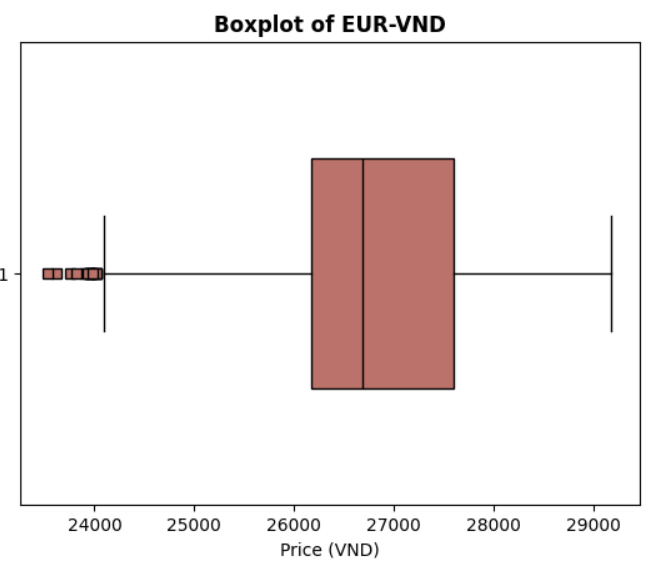
\includegraphics[width=1\textwidth]{Descriptive_statistic/eur_boxplot.png}
    \caption{EUR-VND price's boxplot}
    \label{fig:1}
    \end{minipage}
    \hfill
    \begin{minipage}{0.23\textwidth}
    \centering
    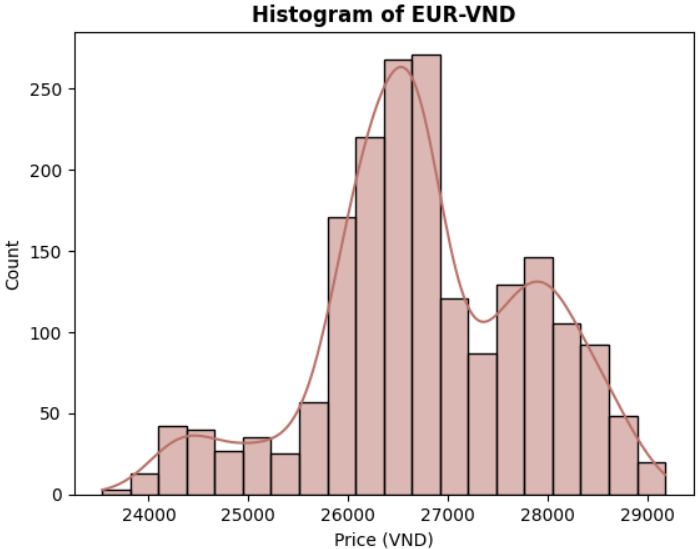
\includegraphics[width=1\textwidth]{Descriptive_statistic/eur_histogram.png}
    \caption{EUR-VND price's histogram}
    \label{fig:2}
    \end{minipage}
\end{figure}
\justify
The descriptive statistics for the EUR-VND exchange rate data are illustrated through both a boxplot and a histogram. The boxplot shows the distribution of selling prices from March 1, 2019, to June 1, 2024, highlighting the median, quartiles, and any potential outliers. This reveals the central tendency and spread of the exchange rates over the specified period. The histogram complements this by displaying the frequency distribution of the EUR-VND selling prices. It indicates that the prices are predominantly clustered around the mean and median values, suggesting a slightly skewed distribution. Together, these visualizations provide a comprehensive overview of the variability and distribution of the EUR-VND selling prices.

\begin{figure}[H]
    \centering
    \begin{minipage}{0.23\textwidth}
    \centering
    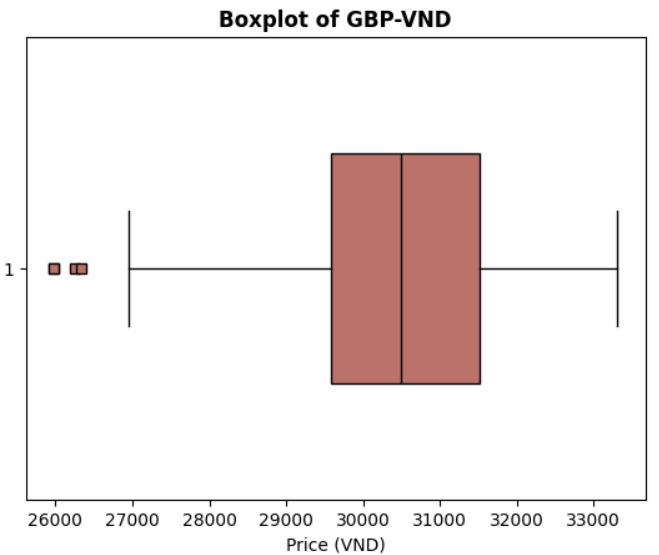
\includegraphics[width=1\textwidth]{Descriptive_statistic/gbp_boxplot.png}
    \caption{GBP-VND price's boxplot}
    \label{fig:1}
    \end{minipage}
    \hfill
    \begin{minipage}{0.23\textwidth}
    \centering
    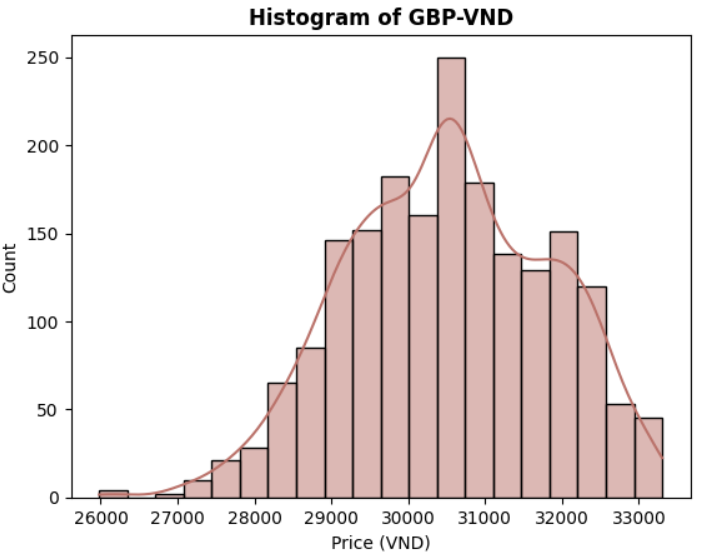
\includegraphics[width=1\textwidth]{Descriptive_statistic/gbp_histogram.png}
    \caption{GBP-VND price's histogram}
    \label{fig:2}
    \end{minipage}
\end{figure}
\justify
For the GBP-VND exchange rate data, the boxplot displays the distribution of selling prices from March 1, 2019, to June 1, 2024, showing the median, quartiles, and potential outliers. The majority of selling prices are concentrated at lower levels, with some higher values contributing to an increased standard deviation. The histogram provides additional insight by depicting the frequency distribution of GBP-VND selling prices, highlighting a right-skewed distribution. Most prices are concentrated at lower levels, with fewer occurrences of higher prices. Together, these visual representations help in understanding the central tendency, variability, and distribution pattern of GBP-VND selling prices.

\begin{figure}[H]
    \centering
    \begin{minipage}{0.23\textwidth}
    \centering
    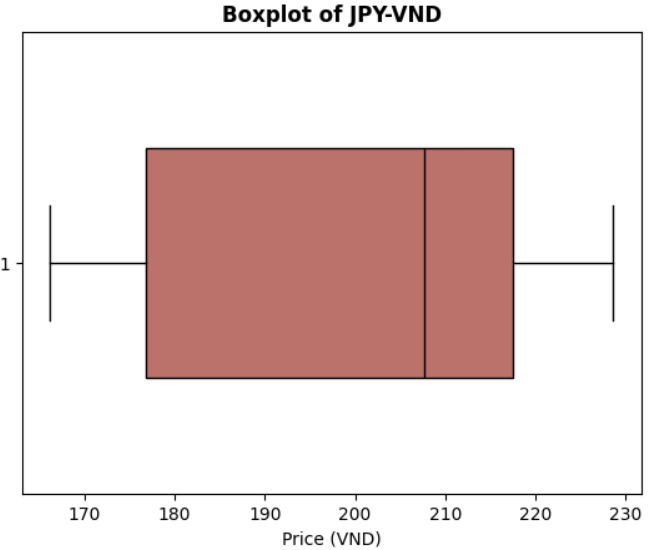
\includegraphics[width=1\textwidth]{Descriptive_statistic/jpy_boxplot.png}
    \caption{JPY-VND price's boxplot}
    \label{fig:1}
    \end{minipage}
    \hfill
    \begin{minipage}{0.23\textwidth}
    \centering
    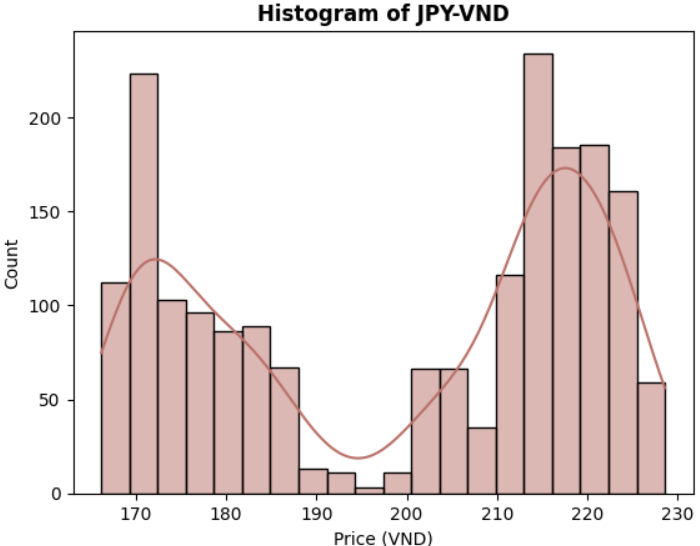
\includegraphics[width=1\textwidth]{Descriptive_statistic/jpy_histogram.png}
    \caption{JPY-VND price's histogram}
    \label{fig:2}
    \end{minipage}
\end{figure}
\justify
The JPY-VND exchange rate data is summarized using a boxplot and a histogram. The boxplot illustrates the distribution of selling prices from March 1, 2019, to June 1, 2024, highlighting the central tendency, spread, and potential outliers. Most values are concentrated at higher price levels, indicating variability and fluctuations in the market selling price of the Japanese Yen to Vietnamese Dong. The histogram shows the frequency distribution of JPY-VND selling prices, indicating instability and variability in the values. Together, these visualizations provide a clear picture of the distribution shape, including any notable skewness or irregular patterns.

\section{Methodology}
\subsection{Linear Regression}
Regression analysis is a tool for building mathematical and statistical models that characterize relationships between a dependent variable and one or more independent, or explanatory, variables, all of which are numerical. This statistical technique is used to find an equation that best predicts the y variable as a linear function of the x variables.
A multiple linear regression model has the form: 
\[Y=\beta_0+\beta_1X_1+\beta_2X_2+\cdots+\beta_kX_k+\varepsilon\]
Where:
\begin{itemize}
	\item $Y$ is the dependent variable (Target Variable).
	\item $X_1, X_2, \ldots, X_k$ are the independent (explanatory) variables.
	\item $\beta_0$ is the intercept term.
	\item $\beta_1,..., \beta_k$ are the regression coefficients for the independent variables.
	\item $\varepsilon$ is the error term. \cite{linear}
 \end{itemize}

 \subsection{AutoRegressive Integrated Moving Average (ARIMA)}
 ARIMA model is a form of regression analysis that gauges the strength of one dependent variable relative to other changing variables. The ARIMA model is used to make predictions about future values of the time series based on its past values. The ARIMA model consists of three parts including Autoregressive (AR), Integrated (I), and Moving Average (MA). \cite{investopedia_arima} \par
\noindent
 The AR component with order p utilizes the preceding p values of the time series for current value prediction. The AR(p) model has the form:
 \[Y_t=\alpha_0+\alpha_1Y_{t-1}+\cdots+\alpha_pY_{t-p}+\epsilon_t\]
Where:
    \begin{itemize}
	\item $Y_t$ is the current observed value.
        \item $Y_{t-1}, \ldots, Y_{t-p}$ are past observed values.
        \item $\alpha_0, \alpha_1, \ldots, \alpha_p$ are regression analysis parameters.
        \item $\epsilon_t$ is the random forecasting error of the current period. The expected mean value is 0.
    \end{itemize}
 Integrated (I) represents the differencing of raw observations, allowing the time series to become stationary.
 \begin{itemize}
    \item First Difference I(1): $dY_t = Y_t - Y_{t-1}$
    \item Second Difference I(2): $dY_t = Y_t - 2Y_{t-2} + Y_{t-3}$
 \end{itemize}
The MA model with order q analyzes the past q forecast errors to anticipate the current value. The MA(q) model has the form:
  \[Y_t=\beta_0+\epsilon_t+\beta_1\epsilon_{t-1}+\cdots+\beta_q\epsilon_{t-q}\]
        Where:
        \begin{itemize}
	    \item $Y_t$ is the current observed value.
            \item $\epsilon_t$ is a random forecasting error of the current period. The expected mean value is 0.
            \item \(\epsilon_{t-1}, \ldots, \epsilon_{t-q}\) are forecast errors.
            \item \(\beta_0, \beta_1, \ldots, \beta_q\) mean values of Y(t) and moving average coefficients.
            \cite{arima_forecasting}
        \end{itemize}
            
\subsection{Exponential Smoothing (ETS)}
Exponential smoothing is one of the most popular models used for demand forecasting in practice. It includes Error, Trend, and Seasonal components, thus being called ‘ETS’.
The trend component (T) represents the tendency to increase or decrease data over time. The seasonal (S) shows the periodic fluctuations at fixed intervals within the data. The fluctuations are affected by specific times of the year like holidays, seasonal changes, or events. The error (E) is also known as residual. It represents the unpredictable or fluctuations in the data that cannot be explained by the trend or seasonal components.
There are three main methods to estimate exponential smoothing, which are: \\
    \indent\textbullet\ Simple exponential smoothing: used when the data has no trend and no seasonal pattern. \\
    \indent\textbullet\ Double exponential smoothing: used for forecasting the time series when the data has a linear trend and no seasonal pattern. \\
    \indent\textbullet\ Triple exponential smoothing: used for forecasting the time series when the data has both linear trend and seasonal pattern. This method is also called Holt-Winters exponential smoothing \cite{ets_triple}
    \begin{align*}
        L_t &= \alpha(Y_t - S_{t-p}) + (1 - \alpha)(L_{t-1} + T_{t-1}) \\
        T_t &= \beta(L_t - L_{t-1}) + (1 - \beta)T_{t-1} \\
        S_t &= \delta(Y_t - L_t) + (1 - \delta)S_{t-p} \\
        \hat{Y}_t &= L_{t-1} + T_{t-1} + S_{t-p}
    \end{align*} 
    \begin{itemize}
      \item $\alpha$, $\beta$, $\gamma$ : smoothing parameters
      \item $Y_t$ : actual data point at time $t$
      \item $S_{t-p}$ : seasonal index at time $t-p$
      \item $T_{t-1}$ : trend at time $t-1$
      \item $L_{t-1}$: the level at time $t-1$
      \item $L$: the level at time $t$
      \item $\hat{Y}_t$: the forecast value at time $t$ \cite{ets_triple_formula}
    \end{itemize}

\subsection{Stacking model} 
The Stacking Model, also known as Ensemble Learning, is a machine learning technique that combines multiple machine learning models to create a more accurate predictive model, flexible and effective approach to solving complex prediction tasks. In general, stacking ensemble learning consists of two phases: base models training phase and meta model training phase:\

In the initial phase, the original data is first split into a training set and a testing set. The training set undergoes training using k-fold cross-validation. This method involves partitioning the training set into k subsets, using k minus one subsets for training the model, and predicting outcomes for the remaining subset.

During the subsequent phase, predictions from the k-fold cross-validation of the base model are aggregated to reconstruct a new training dataset in the original order. The meta model's training set is formed by consolidating these reconstructed datasets from multiple base models. Similarly, predictions from the testing sets of the base models are combined to construct the testing set for the meta model. The meta model is then trained

\begin{figure}[H]
  \centering
  \begin{minipage}{1.0\linewidth}
    \centering
    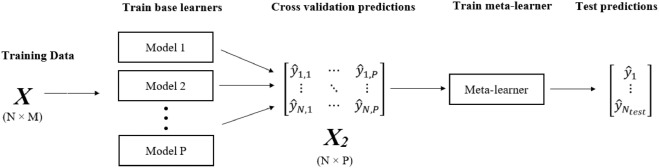
\includegraphics[width=\linewidth]{Figure_algorithm/stackingmodel.jpg}
    \caption{Structure of the Stacking Model \cite{stack_fig}}
  \end{minipage}
\end{figure}

In this report, two models XGBoost, Linear Regerssion  were selected as the base models. The meta-model was chosen as ordinary linear regression. Linear regression is a common choice in regression for the meta-learner

\subsection{XGBoost (For Stacking Model)}
Extreme Gradient Boosting (XGB) is an advanced supervised learning algorithm proposed by Chen and Guestrin. It is based on gradient-boosted decision trees and aims to create a strong learner by aggregating predictions from weak learners using additive training strategies. XGB builds upon gradient-boosted decision trees with a second-order Taylor expansion of the loss function and regularization to prevent overfitting and accelerate convergence. It continuously improves prediction accuracy by iteratively constructing new decision trees to fit residuals from previous predictions, minimizing the difference between predicted and actual values. Its speed advantage makes XGB a preferred choice as a base model for staking model in various studies.\cite{stacking}

\subsection{Recurrent Neural Network (RNN)}
RNN is a type of neural network model designed to handle sequential data. The distinctive feature of RNNs is their ability to maintain information across time steps, allowing them to utilize information from previous steps to influence the processing of the current step. This makes RNNs particularly useful in applications where the order of data is important, such as natural language processing (NLP), machine translation, and time series forecasting. \cite{zargar2021introduction}\\
RNNs operate by processing sequential data and maintaining a hidden state to capture information from previous time steps. The formula for updating the hidden state is:
\[ \alpha_t=\psi_0(W_\alpha_xx_t + W_\alpha_\alpha\alpha_t_-_1 + b_\alpha) \]

Where:\\
    \begin{itemize}
        \item $\alpha_t$ is a hidden layer state at each time step t
        \item $\psi_0$ is the activation function
        \item $W_\alpha_x$ and $W_\alpha_\alpha$ are weight matrices
        \item $x_t$ is an input data
        \item $b_\alpha$ is a bias vector
    \end{itemize}\\

The formula predicts the output at each time t:\\
\[ y_t = \Psi_1(W_y_\alpha\alpha_t + b_y) \]

Where:\\
    \begin{itemize}
        \item $y_t$ is an output data at each time t
        \item $\Psi_1$ is the activation function
        \item $W_y_\alpha$ is weight matrices
        \item $\alpha_t$ is a hidden layer state
        \item $b_y$ is a bias vector
        \cite{zargar2021introduction}
    \end{itemize}

\subsection{Gated Recurrent Unit (GRU)} 
Gated Recurrent Unit (GRU) is a special kind of RNN (Recurrent Neural Network). A GRU cell consists of two gates: the Update gate and the Reset gate. The Update gate operates similarly to the forget gate and input gate of LSTM. It determines how much of the past information to keep and how much new information from the current input to allow into cell state by controlling balance between the previous hidden state and the candidate hidden state \cite{gru_balance}. The Reset gate identifies and forgets unnecessary past information from the GRU network.

The equation of Update gate is as follows:
\begin{align*}
z_t &= \sigma\left( W^{(z)} x_t + U^{(z)} h_{t-1} \right)
\end{align*}

The equation of Reset gate is as follows:
\begin{align*}
r_t &= \sigma\left( W^{(r)} x_t + U^{(r)} h_{t-1} \right)
\end{align*}

Candidate hidden state is calculated from the reset gate and stores information from the past. Its equation is as follows:
\begin{align*}
h_t' &= \tanh(W \mathbf{x}_t + r_t \odot U \mathbf{h}_{t-1})
\end{align*}

The equation of Hidden state is as follows:
\begin{align*}
h_t &= z_t \odot h_{t-1} + (1 - z_t) \odot h_t'  
\end{align*}

Where:\\
    \begin{itemize}
        \item \(h_{t-1}\) represent the output of the previous states
        \item \(z_t\) is the update gate at time \(t\)
        \item \(r_t\) is the reset gate at time \(t\)
        \item \(W_z\), \(W_r\) is the weight matrix
        \item \(h_t\) is the hidden state at time \(t\)
        \item \(h_t'\) is the candidate hidden state at time \(t\)
        \item \(\sigma\) is the logistic sigmoid function \cite{gru_equation} \\
    \end{itemize}\\

\subsection{Long Short-Term Memory (LSTM)} 
The LSTM (Long Short-Term Memory) model, a specialized form of Recurrent Neural Network (RNN), was introduced by Hochreiter and Schmidhuber in 1997 to tackle the issue of long-term dependencies. It consists of a chain-like structure with up to four interacting layers. Each LSTM includes a cell state and three gates: forget, input, and output. These gates are controlled by sigmoid layers.\cite{zargar2021introduction}
\begin{figure}[H]
  \centering
  \begin{minipage}{0.8\linewidth}
    \centering
    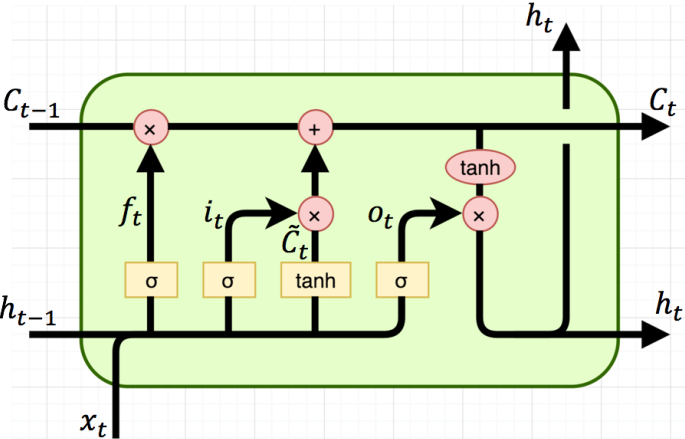
\includegraphics[width=\linewidth]{Figure_algorithm/lstm (1).png}
    \caption{Structure of the LSTM model \cite{lstm_fig}}
  \end{minipage}
\end{figure}
The initial step of the LSTM model involves the forget gate layer, which decides what information to discard from the cell state. The formula for the forget gate is:
\[ f_t = \sigma(W_f \cdot [h_{t-1}, x_t] + b_f) \]
Where:
\begin{itemize}
    \item \( \sigma \) is the sigmoid function.
    \item \( W_f \) and \( b_f \) are the weights and bias of the forget gate layer.
\end{itemize}

Subsequent steps determine which information is stored in and updates the cell state. This involves an input gate layer and a vector of values from the tanh layer. The formulas for the input gate and state update are:
\begin{align*}
    i_t & = \sigma(W_i \cdot [h_{t-1}, x_t] + b_i) \\
    \tilde{C}_t & = \tanh(W_C \cdot [h_{t-1}, x_t] + b_C) \\
    C_t & = f_t \cdot C_{t-1} + i_t \cdot \tilde{C}_t
\end{align*}
Where:
\begin{itemize}
    \item \( C_{t-1} \) and \( C_t \) are the cell states at time \( t-1 \) and \( t \)
    \item \( W_i, W_C \), and their respective variables are weights,
\end{itemize}

Finally, the output \( h_t \) is determined by the output gate and the cell state. The formula for the output gate is:
\begin{align*}
    o_t & = \sigma(W_o \cdot [h_{t-1}, x_t] + b_o) \\
    h_t & = o_t \cdot \tanh(C_t)
\end{align*}

\subsection{Multilayer Perceptron (MLP)}
MLP is a type of artificial neural network that belongs to the feed-forward neural network group. It consists of multiple layers: an input layer, one or more hidden layers, and an output layer. Each neuron in an MLP uses a nonlinear activation function, such as the sigmoid, ReLU, or tanh function. These neurons are fully connected, meaning each neuron in one layer is connected to every neuron in the adjacent layer. MLP can learn and model nonlinear relationships between inputs and outputs, making it effective for many complex problems. \cite{mlp}
\begin{figure}[H]
  \centering
  \begin{minipage}{0.8\linewidth}
    \centering
    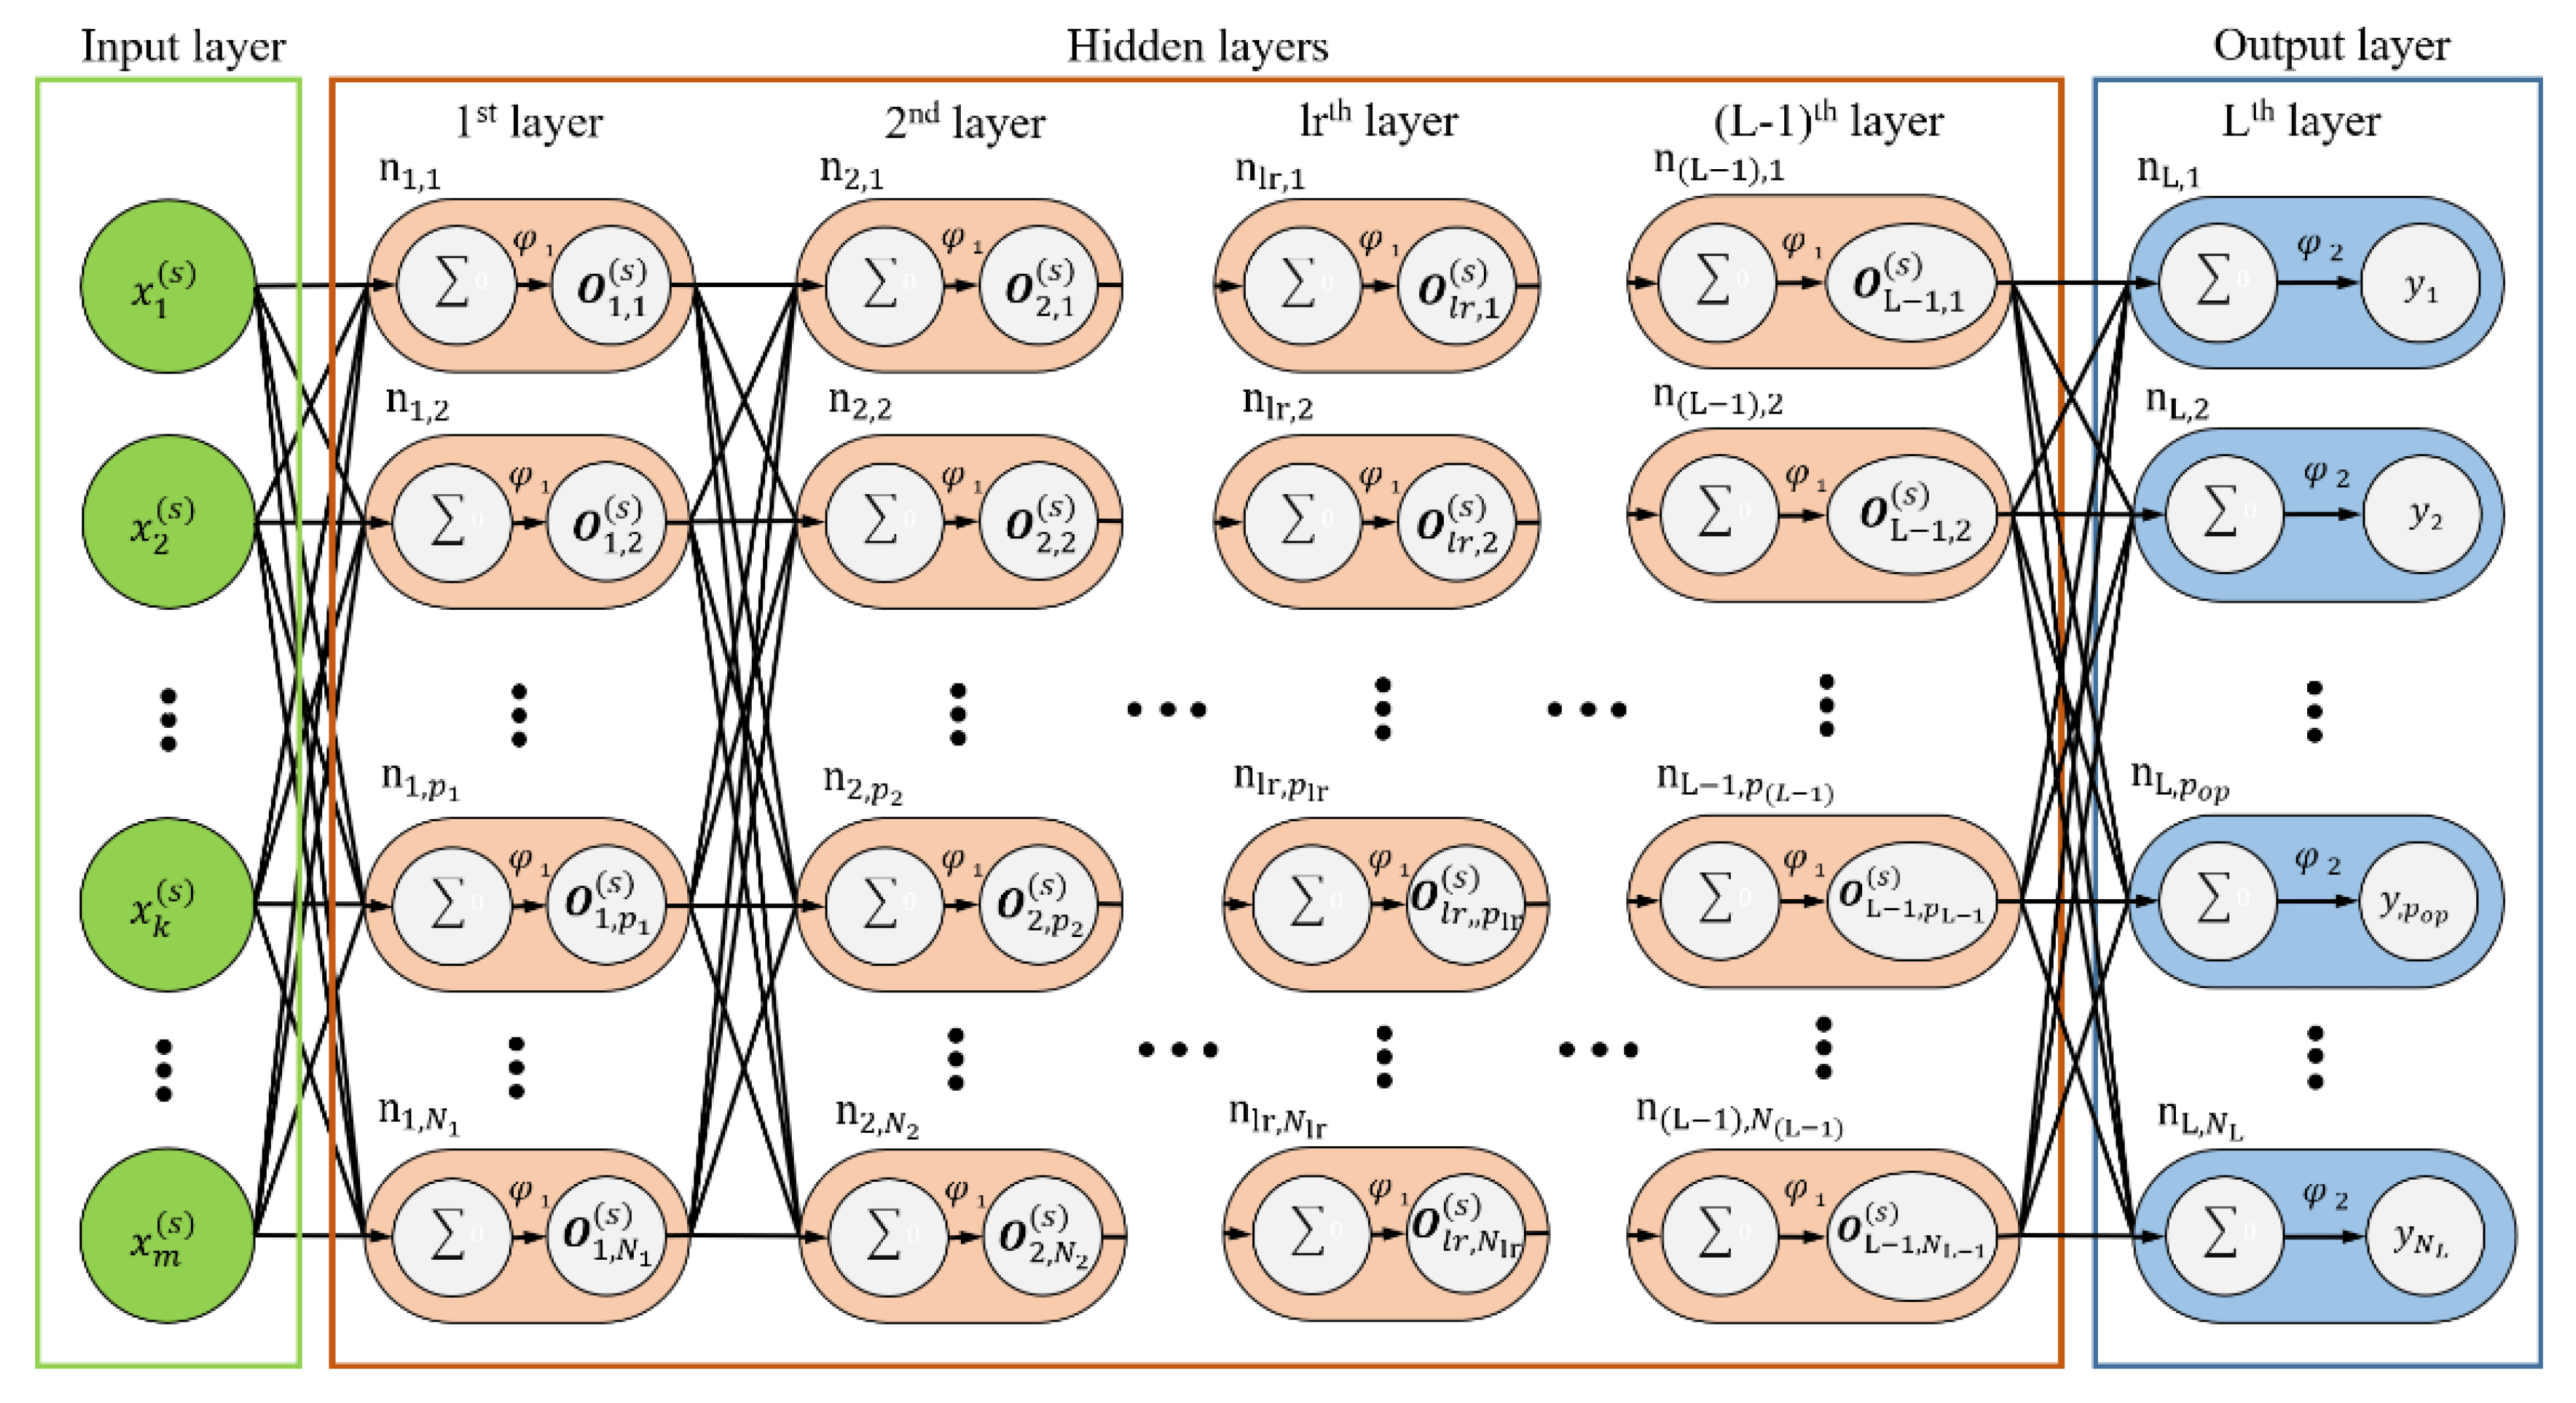
\includegraphics[width=\linewidth]{Figure_algorithm/mlp.png}
    \caption{Structure of the MLP model \cite{mlp_image}}
    \label{fig_mlp}
  \end{minipage}
\end{figure}
The formula to calculate the input values of a layer (except the input layer):
\[ z^{(l)} = W^{(l) T}\alpha^{(l-1)} + b^{(l)} \]
Where:
    \begin{itemize}
        \item $z^{(l)}$ is a matrix containing the input values for each neuron in layer (l)
        \item $W^{(l)}$ is a matrix containing the connection weights between neurons in layer (l-1) and neurons in layer (l)
        \item $\alpha^{(l-1)}$ is a matrix containing the output values of layer (l-1) and serves as the input for layer (l). For the layer immediately following the input layer, it will be replaced by matrix X
        \item $b^{(l)}$ is a matrix containing the threshold values for each neuron in layer (l)
    \end{itemize}
        
When the input value exceeds the threshold, meaning the neuron's z value is greater than 0, the neuron will produce an output value. The formula to calculate the output of a layer (except the input layer):
\[ \alpha^{(l)} = f(z^{(l)}) \]
Where:
    \begin{itemize}
        \item $\alpha^{(l)}$ is a matrix containing the output values of each neuron belonging to layer l
        \item  $f()$ is an activation function, such as the sigmoid, ReLU, or tanh function
    \end{itemize}\\
    
\section{Result}
\subsection{Evaluation Methods}
\textbf{Mean Percentage Absolute Error} (MAPE): is the average percentage error in a set of predicted values.\\
\[MAPE=\frac{100\%}{n}  \sum_{i=1}^{n} |\frac{y_i-\hat{y_i}}{y_i}|\]\\
\textbf{Root Mean Squared Error} (RMSE): is the square root of the average value of squared error in a set of predicted values.\\
\[RMSE=\sqrt{\frac{1}{n} \sum_{i=1}^{n}(\hat{y_i}-y_i )^2}\]\\
\textbf{Mean Absolute Error} (MAE): is a measure of the average difference between predicted values and actual values in a dataset.\\
\[MAE = \frac{1}{n} \sum_{i=1}^{n} |y_i - \hat{y_i}| \]
Where: \\
	\indent\textbullet\ \(n\) is the number of observations in the dataset.\\
	\indent\textbullet\ \(y_i\)  is the true value.\\
	\indent\textbullet\ \(\hat{y_i}\) is the predicted value.
        \cite{sefidian_guide}
        
\subsection{Evaluation Tables} 

\begin{table}[H]
    \centering
    \begin{tabular}{|c|c|c|c|c|}
         \hline
         \multicolumn{5}{|c|}{\textbf{EUR-VND Dataset's Evaluation}}\\
         \hline
         \centering Model & Train:Test & RMSE & MAPE (\%) & MAE\\
         \hline
         \multirow{2}{*}{LR} & 7:3 &1261.17 &3.632 &993.698 \\ & 8:2 & 1447.716 & 4.61 & 1267.462 \\& 9:1 & 1604.473 & 5.581 & 549.852 \\
         \hline
         \multirow{2}{*}{ARIMA} & 7:3 & 1830.875 & 6.224 & 1687.944 \\ & 8:2 & 987.512 & 2.998 & 825.492 \\ & 9:1 & 610.009&1.789 & 499.686\\
         \hline
         \multirow{2}{*}{ETS} & 7:3 & 1631.753 & 5.547 & 1504.453 \\ & 8:2 & 532.582&1.5499&426.105 \\& 9:1 & 236.536 & 0.696& 192.593 \\
         \hline
         \multirow{2}{*}{Stacking} & 7:3 & 1443.383 & 4.991 & 1323.673 \\ & 8:2 &698.075&2.066&553.825\\& 9:1 & 822.191 & 2.511 & 700.179 \\
         \hline
         \multirow{2}{*}{RNN} & \textbf{7:3} & \textbf{93.655} & \textbf{0.252} & \textbf{67.515} \\ & \textbf{8:2} & \textbf{92.962} & \textbf{0.254} & \textbf{69.081} \\ & \textbf{9:1} & \textbf{81.738} & \textbf{0.205} &\ \textbf{56.667} \\
         \hline
         \multirow{2}{*}{GRU} & 7:3 & 95.492 & 0.259 & 69.448 \\ & 8:2 & 93.5 & 0.253 & 68.955 \\ & 9:1 & 82.348 & 0.204 & 56.4306 \\
         \hline
         \multirow{2}{*}{LSTM} & 7:3 & 101.108 &0.287 &77.325\\ & 8:2 &127.054& 0.367 & 100.78 \\&9:1&95.397 &0.26&72.617 \\
         \hline
         \multirow{2}{*}{MLP} & 7:3 &107.318&0.304&81.334 \\ & 8:2 & 103.057&0.293&80.011 \\ & 9:1 & 88.979&0.227&62.903\\
         \hline
    \end{tabular}
    \caption{EUR-VND Dataset's Evaluation}
    \label{vcbresult}
\end{table}

Table 2 presents the evaluation metrics for different models applied to the EUR-VND (Euro to Vietnamese Dong) dataset. Based on the evaluation metrics in the table, including RMSE (Root Mean Square Error), MAPE (Mean Absolute Percentage Error), and MAE (Mean Absolute Error), we can determine which algorithm performs best for each dataset split ratio (7:3, 8:2, 9:1) of the EUR-VND dataset. Specifically, for the 7:3 split ratio, the RNN model performs best with RMSE of 110.09, MAPE of 0.252\%, and MAE of 67.515. For the 8:2 split ratio, the RNN continues to show superior performance with RMSE of 91.017, MAPE of 0.204\%, and MAE of 56.667. Lastly, for the 9:1 split ratio, the RNN model maintains its leading position with RMSE of 81.738, MAPE of 0.205\%, and MAE of 56.667. The RNN model delivers the best results across all three split ratios (7:3, 8:2, 9:1) based on the evaluation metrics mentioned. This indicates that RNN is the most effective algorithm for predicting EUR-VND exchange rates in different data split scenarios.

\begin{table}[H]
    \centering
    \begin{tabular}{|c|c|c|c|c|}
         \hline
         \multicolumn{5}{|c|}{\textbf{GBP-VND Dataset's Evaluation}}\\
         \hline
         \centering Model & Train:Test & RMSE & MAPE (\%) & MAE\\
         \hline
         \multirow{2}{*}{LR} &7:3&1261.17 &3.632 &993.698\\ &\ 8:2 & 1447.716& 4.61 & 1267.462 \\&9:1 &1604.473 & 5.581 &1549.852 \\
         \hline
         \multirow{2}{*}{ARIMA} &7:3 & 2266.597 &6.304 &1974.25 \\ & 8:2 & 1610.114 & 4.373 & 1390.125 \\&9:1&1112.536 &3.071 & 991.12\\
         \hline
         \multirow{2}{*}{ETS} & 7:3 & 1751.462&5.0491&1569.855 \\ & 8:2 & 1081.92&3.0195&952.128 \\& 9:1& 314.804 & 0.817 & 261.519\\
         \hline
         \multirow{2}{*}{Stacking Model}&7:3&1373.337&3.719&1160.102\\&8:2&967.166&2.466&780.687\\&9:1&1416.977&3.957&1276.006 \\
         \hline
         \multirow{2}{*}{RNN} & \textbf{7:3} & \textbf{125.438} & \textbf{0.297} & \textbf{90.847} \\ & 8:2 & 122.789 & 0.294 & 92.395 \\ & 9:1 & 105.797 & 0.234 & 75.146 \\
         \hline
         \multirow{2}{*}{GRU} & 7:3 & 124.999 & 0.286 & 87.592 \\ & \textbf{8:2} & \textbf{128.489} & \textbf{0.3153} & \textbf{99.099} \\ & \textbf{9:1} & \textbf{106.643} & \textbf{0.232} &\ \textbf{74.63} \\
         \hline
         \multirow{2}{*}{LSTM} &7:3 &147.362&0.374&115.568 \\ & 8:2 &122.03&	0.293&	92.348 \\&9:1&121.924&0.291 &94.226\\
         \hline
         \multirow{2}{*}{MLP} & 7:3 & 150.163	&0.38&	116.529 \\ &8:2 & 157.483&	0.414&	130.517\\ & 9:1 & 126.791&	0.296&	95.064\\
         \hline
    \end{tabular}
    \caption{GBP-VND Dataset's Evaluation}
    \label{mbbresult}
\end{table}

Table 3 presents the evaluation metrics for different models applied to the GBP-VND (British Pound to Vietnamese Dong) dataset. Based on the evaluation metrics in the table, including RMSE (Root Mean Square Error), MAPE (Mean Absolute Percentage Error), and MAE (Mean Absolute Error), we can determine which algorithm performs best for each dataset split ratio (7:3, 8:2, 9:1) of the GBP-VND dataset. Specifically, for the 7:3 split ratio, the RNN model performs best with RMSE of 125.438, MAPE of 0.297\%, and MAE of 90.34. For the 8:2 split ratio, the GRU model shows superior performance with RMSE of 105.797, MAPE of 0.234\%, and MAE of 75.146. Lastly, for the 9:1 split ratio, the GRU model maintains its leading position with RMSE of 93.921, MAPE of 0.246\%, and MAE of 70.453. The GRU model delivers the best results for the 8:2 and 9:1 split ratios, while the RNN model performs best for the 7:3 split ratio based on the evaluation metrics mentioned. This indicates that GRU is the most effective algorithm for predicting GBP-VND exchange rates in the 8:2 and 9:1 data split scenarios, while RNN is optimal for the 7:3 split ratio.

\begin{table}[H]
    \centering
    \begin{tabular}{|c|c|c|c|c|}
         \hline
         \centering Model & Train:Test & RMSE & MAPE (\%) & MAE\\
         \hline
         \multirow{2}{*}{LR} &7:3&1261.170 &3.632&993.698 \\ &8:2 & 1447.716&4.61&1267.462 \\&9:1 & 1604.473	&5.581	&1549.852 \\
         \hline
         \multirow{2}{*}{ARIMA} & 7:3 & 10.529 & 5.592 & 9.836 \\ & 8:2 & 9.014 & 5.089 & 8.656 \\& 9:1& 5.955 &3.239&5.565 \\
         \hline
         \multirow{2}{*}{ETS} & 7:3 & 10.054&5.298&9.326 \\ & 8:2 &5.459&2.853 &4.852\\& 9:1 &5.883&3.194&5.488 \\
         \hline
         \multirow{2}{*}{Stacking Model} & 7:3 & 27.438	&13.326	&23.19 \\& 8:2 &13.681	&7.595&	12.946\\ & 9:1&6.886 &3.577 &6.127\\
         \hline
         \multirow{2}{*}{RNN} & \textbf{7:3} & \textbf{1.119} & \textbf{0.444} &\textbf{0.779} \\ &8:2 & 0.867 &0.369 & 0.629 \\ & 9:1 & 0.87 & 0.396 & 0.675 \\
         \hline
         \multirow{2}{*}{GRU} & 7:3 & 1.044 & 0.408 & 0.714 \\ & 8:2 & 0.86 & 0.355 & 0.607 \\ &9:1 &0.788& 0.332 & 0.567 \\
         \hline
         \multirow{2}{*}{LSTM} &\ 7:3 &\ 1.267	&0.552	&0.957  \\&\textbf{8:2}&\textbf{0.99} &\textbf{0.43} &\textbf{0.733} \\ &\textbf{9:1} &\textbf{1.115}&	\textbf{0.494}&	\textbf{0.839}\\
         \hline
         \multirow{2}{*}{MLP} & 7:3 &1.424&	0.572&1.003 \\ &8:2 &1.102&	0.501&0.856\\ & 9:1 &0.917&	0.393	&0.671 \\
         \hline
    \end{tabular}
    \caption{JPY-VND Dataset's Evaluation}
    \label{mbbresult}
\end{table}

Table 4 presents the evaluation metrics for different models applied to the JPY-VND (Japanese Yen to Vietnamese Dong) dataset. Based on the evaluation metrics in the table, including RMSE (Root Mean Square Error), MAPE (Mean Absolute Percentage Error), and MAE (Mean Absolute Error), we can determine which algorithm performs best for each dataset split ratio (7:3, 8:2, 9:1) of the JPY-VND dataset. Specifically, for the 7:3 split ratio, the RNN model performs best with RMSE of 1.686, MAPE of 0.537\%, and MAE of 0.724. For the 8:2 split ratio, the LSTM model shows superior performance with RMSE of 0.99, MAPE of 0.434\%, and MAE of 0.433. Lastly, for the 9:1 split ratio, the LSTM model maintains its leading position with RMSE of 1.115, MAPE of 0.494\%, and MAE of 0.738. The LSTM model delivers the best results for the 8:2 and 9:1 split ratios, while the RNN model performs best for the 7:3 split ratio based on the evaluation metrics mentioned. This indicates that LSTM is the most effective algorithm for predicting JPY-VND exchange rates in the 8:2 and 9:1 data split scenarios, while RNN is optimal for the 7:3 split ratio.

\subsection{Optimal Cases Visualization} 

\begin{figure}[H]
  \centering
  \begin{minipage}{0.8\linewidth}
    \centering
    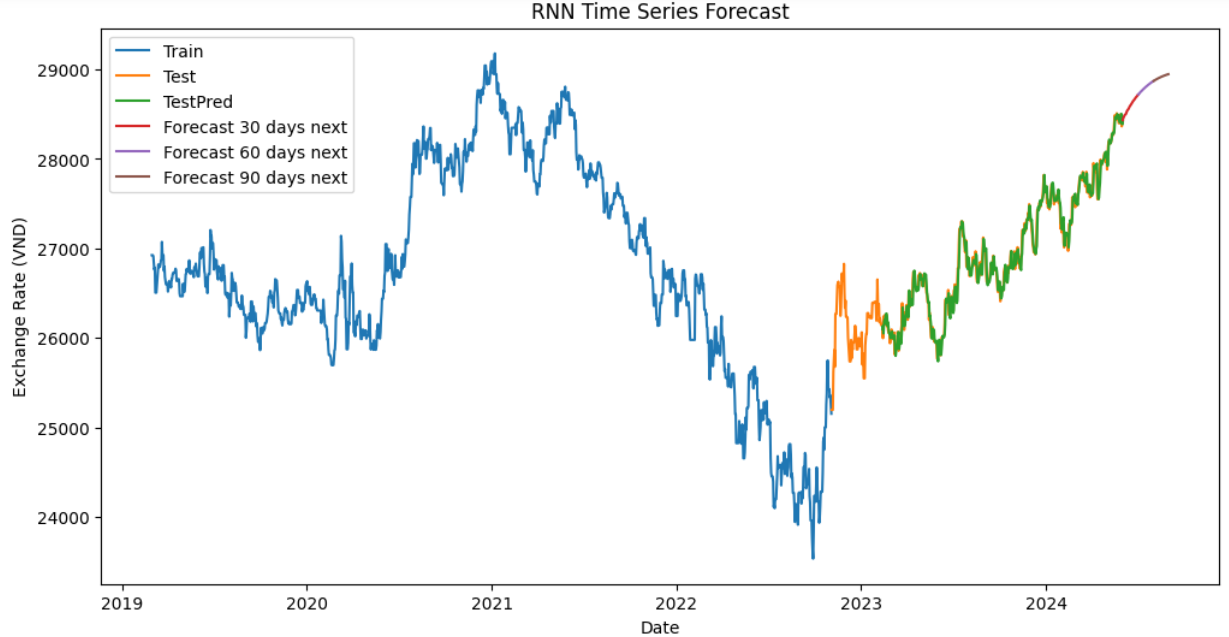
\includegraphics[width=\linewidth]{RNN/rnn_eur_73.png}
    \caption{RNN Prediction Model for EUR-VND Dataset with 7:3 Split Ratio}
    \label{fig26}
  \end{minipage}
\end{figure}
\begin{figure}[H]
  \centering
  \begin{minipage}{0.8\linewidth}
    \centering
    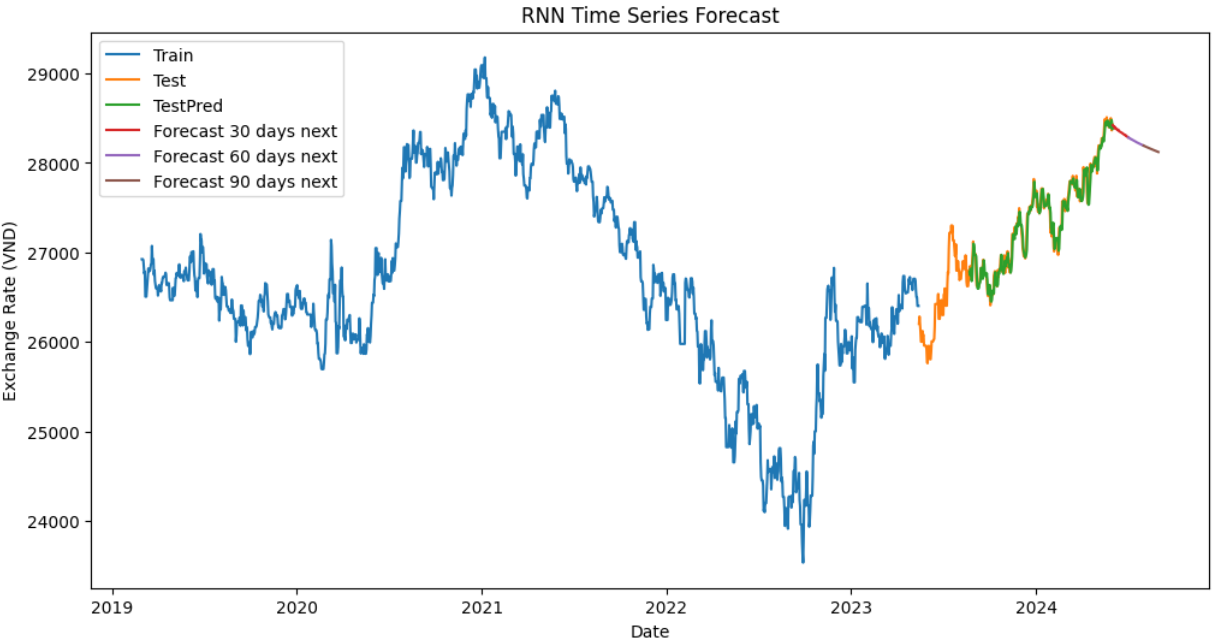
\includegraphics[width=\linewidth]{RNN/rnn_eur_82.png}
    \caption{RNN Prediction Model for EUR-VND Dataset with 8:2 Split Ratio}
    \label{fig27}
  \end{minipage}
\end{figure}
\begin{figure}[H]
  \centering
  \begin{minipage}{0.8\linewidth}
    \centering
    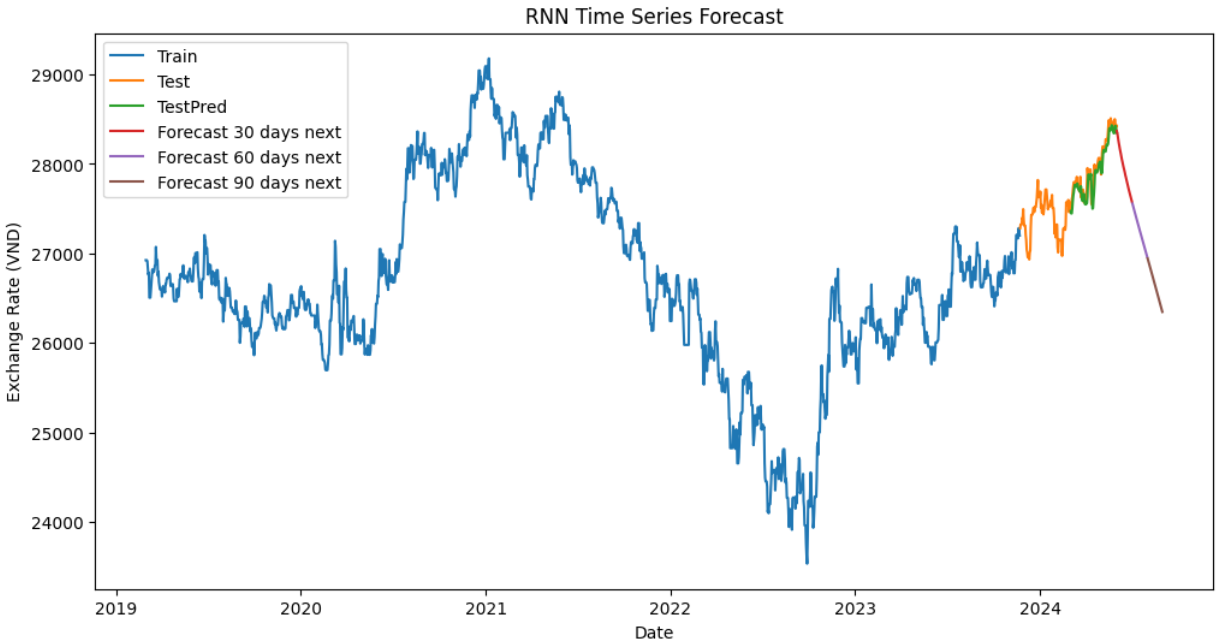
\includegraphics[width=\linewidth]{RNN/rnn_eur_91.png}
    \caption{RNN Prediction Model for EUR-VND Dataset with 9:1 Split Ratio}
    \label{fig28}
  \end{minipage}
\end{figure}
\begin{figure}[H]
  \centering
  \begin{minipage}{0.8\linewidth}
    \centering
    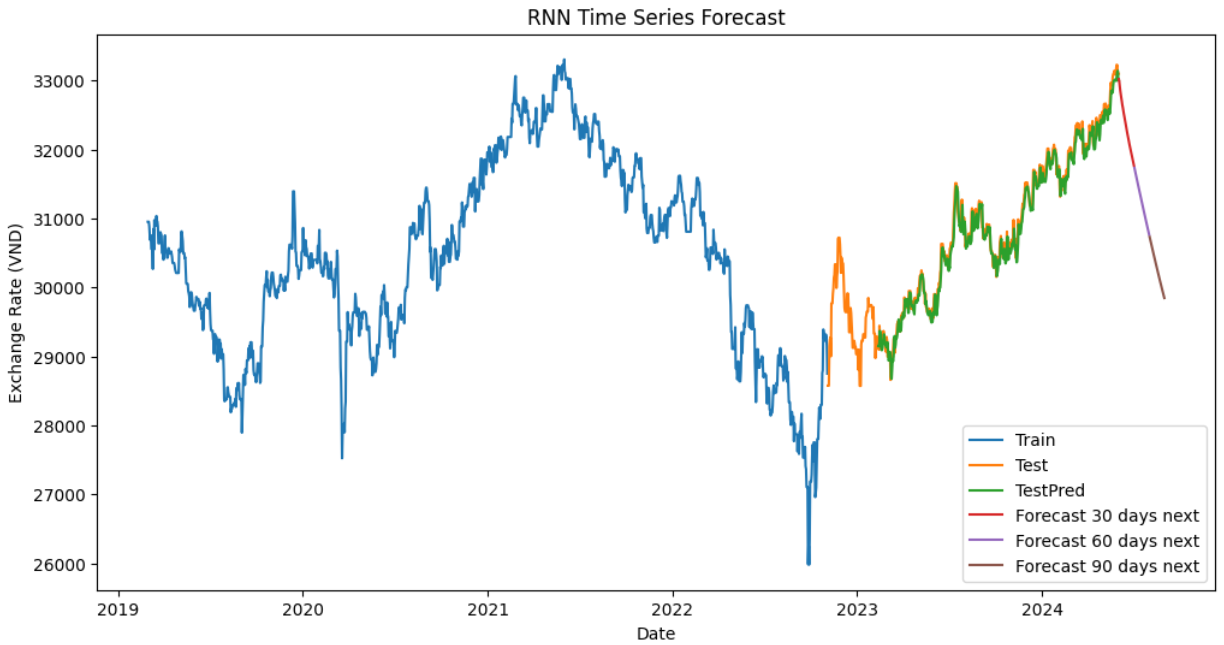
\includegraphics[width=\linewidth]{RNN/rnn_gbp_73.png}
    \caption{RNN Prediction Model for GBP-VND Dataset with 7:3 Split Ratio}
    \label{fig29}
  \end{minipage}
\end{figure}
\begin{figure}[H]
  \centering
  \begin{minipage}{0.8\linewidth}
    \centering
    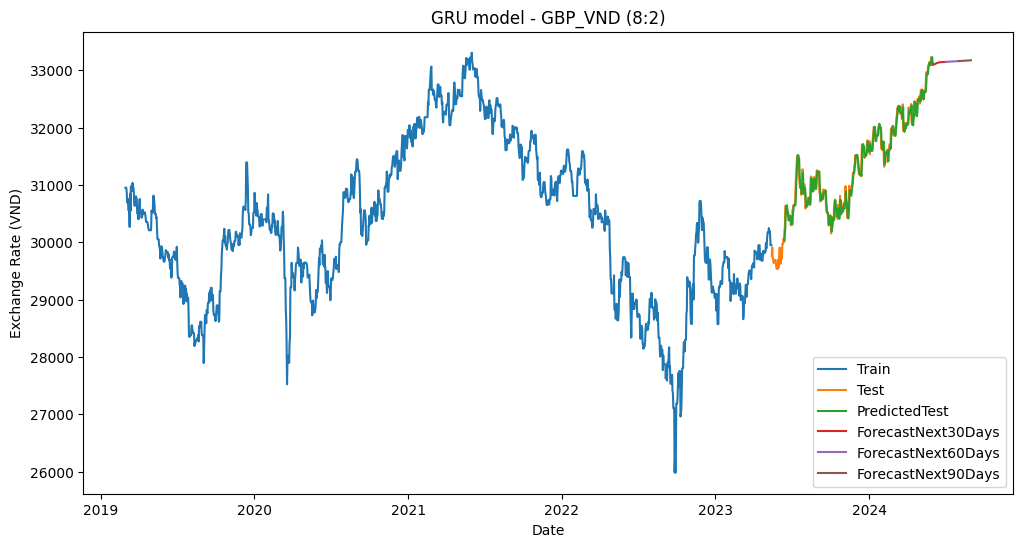
\includegraphics[width=\linewidth]{GRU/GRU_gbp_82.png}
    \caption{GRU Prediction Model for GBP-VND Dataset with 8:2 Split Ratio}
    \label{fig30}
  \end{minipage}
\end{figure}
\begin{figure}[H]
  \centering
  \begin{minipage}{0.8\linewidth}
    \centering
    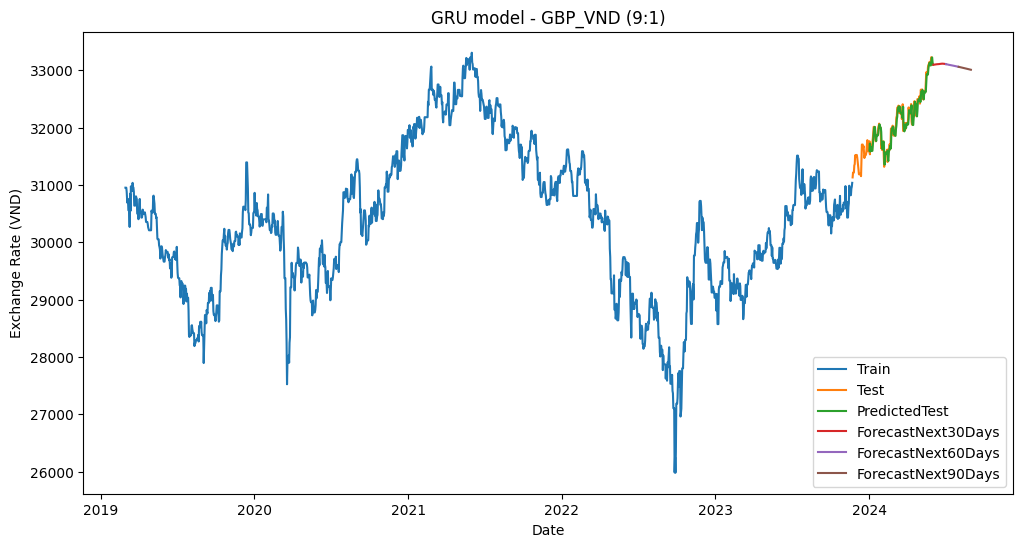
\includegraphics[width=\linewidth]{GRU/GRU_gbp_91.png}
    \caption{GRU Prediction Model for GBP-VND Dataset with 9:1 Split Ratio}
    \label{fig31}
  \end{minipage}
\end{figure}
\begin{figure}[H]
  \centering
  \begin{minipage}{0.8\linewidth}
    \centering
    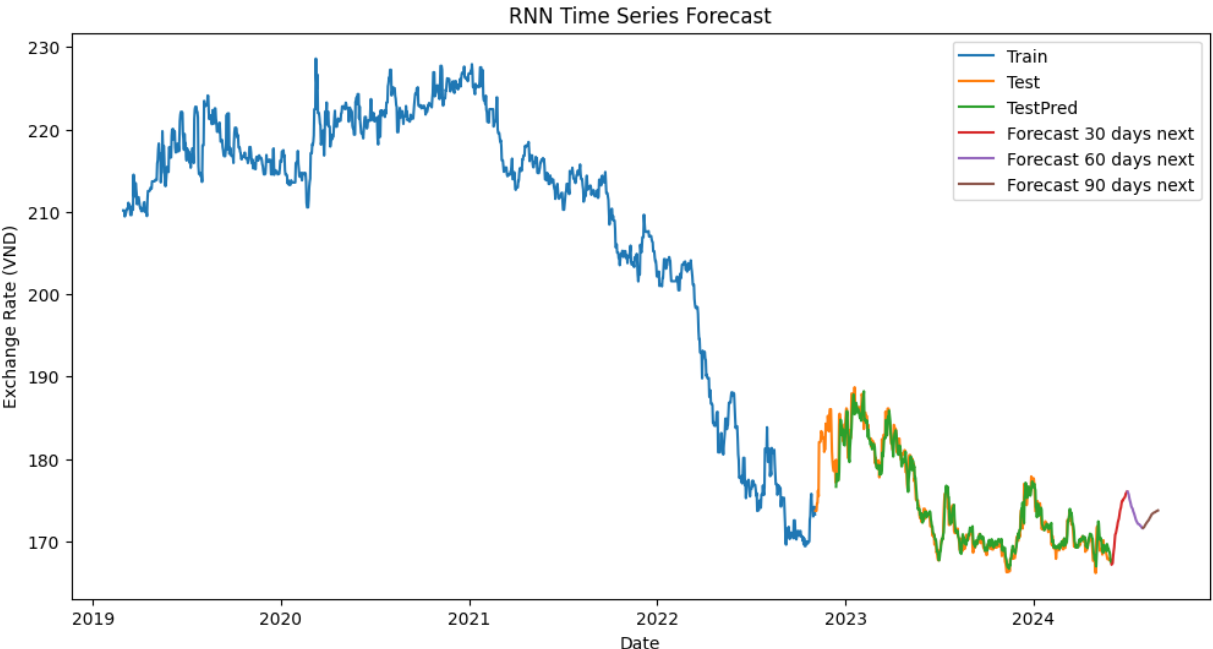
\includegraphics[width=\linewidth]{RNN/rnn_jpy_73.png}
    \caption{RNN Prediction Model for JPY-VND Dataset with 7:3 Split Ratio}
    \label{fig32}
  \end{minipage}
\end{figure}
\begin{figure}[H]
  \centering
  \begin{minipage}{0.8\linewidth}
    \centering
    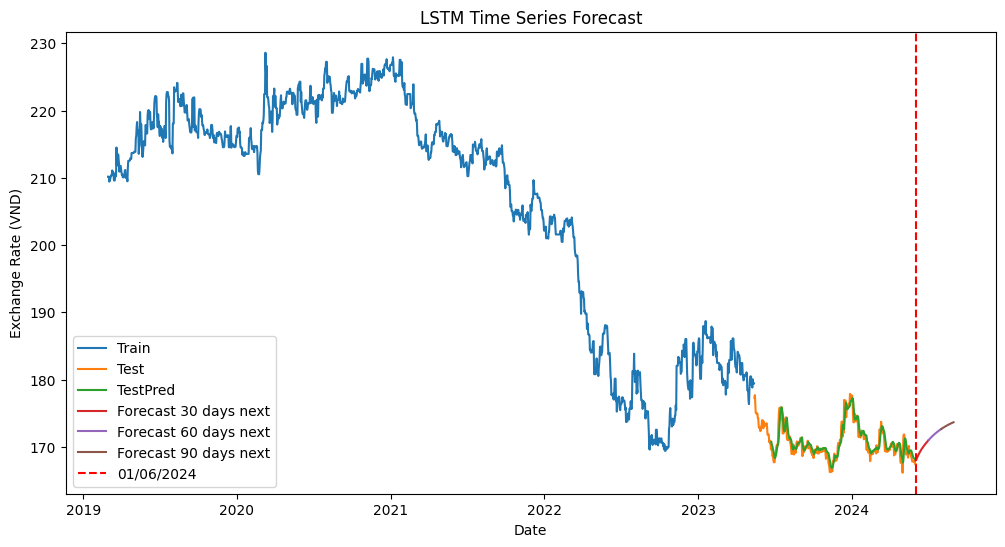
\includegraphics[width=\linewidth]{LSTM/lstm_jpy82.png}
    \caption{LSTM Prediction Model for JPY-VND Dataset with 8:2 Split Ratio}
    \label{fig33}
  \end{minipage}
\end{figure}
\begin{figure}[H]
  \centering
  \begin{minipage}{0.8\linewidth}
    \centering
    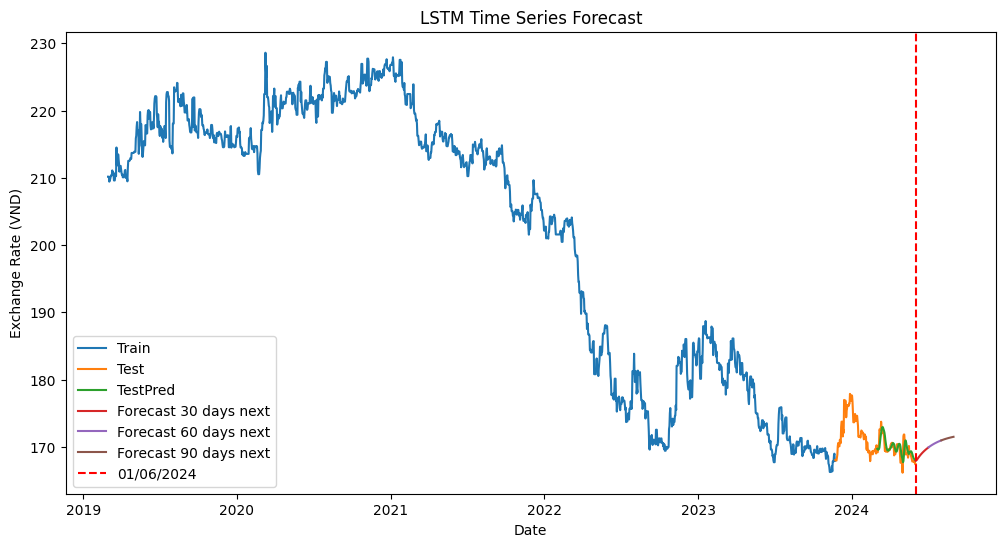
\includegraphics[width=\linewidth]{LSTM/lstm_jpy91.png}
    \caption{LSTM Prediction Model for JPY-VND Dataset with 9:1 Split Ratio}
    \label{fig33}
  \end{minipage}
\end{figure}

\section{Conclusion}
\subsection{Summary}

In the study, we developed and evaluated several models for forecasting currency prices, leveraging different statistical, deep learning, and machine learning techniques. The eight models used are Linear Regression (LR), ARIMA, Exponential Smoothing (ETS), Long Short Term Memory (LSTM), Recurrent Neural Network (RNN), Gated Recurrent Unit (GRU), Stacking Model, and Multi-layer Perceptron (MLP). The assessment and comparison of forecasting methods highlighted that each technique possessed its own advantages and drawbacks. We used metrics like RMSE, MAE, and MAPE to evaluate model accuracy. By comparing these evaluation metrics, we determined that the RNN and LSTM models are well-suited for forecasting currency prices. 

These models performed more accurately in predicting future prices than the others. Specifically, for the EUR-VND dataset, the RNN model demonstrated superior performance with a 7:3 split ratio, while the LSTM model excelled with 8:2 and 9:1 split ratios. For the GBP-VND dataset, the GRU model was the best for 8:2 and 9:1 split ratios, whereas the RNN model performed best for the 7:3 split ratio. Similarly, for the JPY-VND dataset, the LSTM model delivered the best results for 8:2 and 9:1 split ratios, with the RNN model being optimal for the 7:3 split ratio.
 
\subsection{Future Plans}
\subsection{Future Plans}
The above algorithms have demonstrated promising results in forecasting currency prices. However, it is necessary to enhance the models to achieve greater accuracy and reliability. To accomplish this, several key strategies can be implemented:
\begin{itemize}
    \item \textbf{Enhancing the accuracy of the models:} This includes improving data quality by cleaning and preprocessing data before it is used in the models.
    \item \textbf{Combine various Neural Network methods:} Accuracy can be enhanced by combining different Neural Network techniques. For instance, a CNN-LSTM hybrid model can be effective, as CNN extracts temporal features from the data while LSTM captures long-term dependencies.
    \item \textbf{Research on Advanced prediction models:} Exploring new advanced techniques such as Deep Learning and Reinforcement Learning can help build more sophisticated and accurate prediction models.
    \item \textbf{Build a website:} Developing a website that integrates various neural network models to forecast currency prices. The website can display real-time currency prices and provide features to view and forecast future prices, ensuring real-time data processing.
\end{itemize}

\section*{Acknowledgment}
\addcontentsline{toc}{section}{Acknowledgment}
Firstly, we send our deepest appreciation to both \textbf{Assoc. Prof. Dr. Nguyen Dinh Thuan} and \textbf{Mr. Nguyen Minh Nhut} for their invaluable guidance and insightful lessons during the research process. Their constructive feedback has enriched our research and we have not only knowledge, but also the skills needed for our careers. 
\\Secondly, this research would not have been done without the efforts and contributions of our teammates. Thank you for your continued efforts. 
\\Finally, we would like to extend our heartfelt thanks to everyone involved for their invaluable assistance, encouragement, and belief in our research. Thank you all for your invaluable assistance and encouragement.

\EOD
\printbibliography
\end{document}
